\chapter{Proposed Work and Planning}
\label{chapter:PWP}

\quad The proposed work for the dissertation consists in the development of an Auto-Tuning Software for the Deep Versat Architecture
while connected to the IOB-RV32 CPU.
The compiler's propose is to be able to run any state of the art CNN on the Deep Versat system with no effort on the user side. For the proof of concept
stage, Darknet and Caffe will be the frameworks chosen to be compatible with this compiler.

Deep Versat has customizable FU amounts and options, so the compiler must be able to change the datapath based on the Deep Versat Configuration.
  

\section{Hardware System}

\quad For the Auto-Tuning Software to be able to model CNNs for Deep Versat, the System needs to access External Memory for the weights and inputs as for state of the art network like 
Yolov3~\cite{yolov3} has 107 total layers with weight size of 236MB. That amount can not be stored in BRAMs so the IOB-RV32 will have
to load from memory (RAM) to Deep Versat and vice-versa.

INPUT IMAGE HERE 


\subsection{Acceleration on Deep Versat}

\quad Some of the activation functions discussed in chapter \ref{chapter:cnn} will have to be processed in software on the core unless
custom Functional Units are made for each function. Convolutional,Fully Connected,Shortcut and Route layers can be implemented on Deep Versat without
any FU changes. How much it will be accelerated is based on number of cores and MACs available. Pooling needs adaptation in Hardware to run them, if not implemented, run on the RISC-V core.


\newpage
\section{Software Proposal}


\begin{figure}[!htbp]
    \centering
    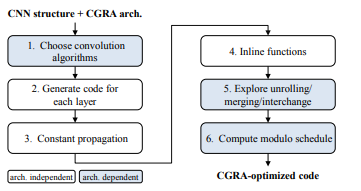
\includegraphics[width=0.8\textwidth]{Figures/cgraopt.png}
    \caption{Optimizing Runs on CGRA. Taken from ~\cite{cgraopt}}
    \label{figure:cgraopt}
\end{figure}

\quad To build a CNN model for Versat, a parser from Configuration file to layer is needed. For darknet~\cite{darknet}, the parser can be re-used.
For Caffe, a new one would need to be built so the output of the parser is equal to other frameworks for the same CNN network.
The objective to be accomplished is to support all Caffe possible layers and Darknet's layers.
After parsing, the Versat dataflow and runs for each type of layer will be defined depending on current silicon set up of the CGRA. Then,
the C code with the Versat runs will be written. In~\ref{figure:cgraopt}, a CGRA optimization flow for CNN is presented.


\section{Planning}

\quad In fig~\ref{figure:gant} is presented a GANT chart with the proposed schedule of the planned work.

\begin{figure}[!htbp]
    %\centering
    \includegraphics[width=1\textwidth]{Figures/gant2.png}
    \caption{GANT chart of Proposed Work}
    \label{figure:gant}
\end{figure}





